
\begin{figure}[!h]
\vspace{-20pt}
\centering
\begin{subfigure}[b]{0.95\textwidth}
	\centering
	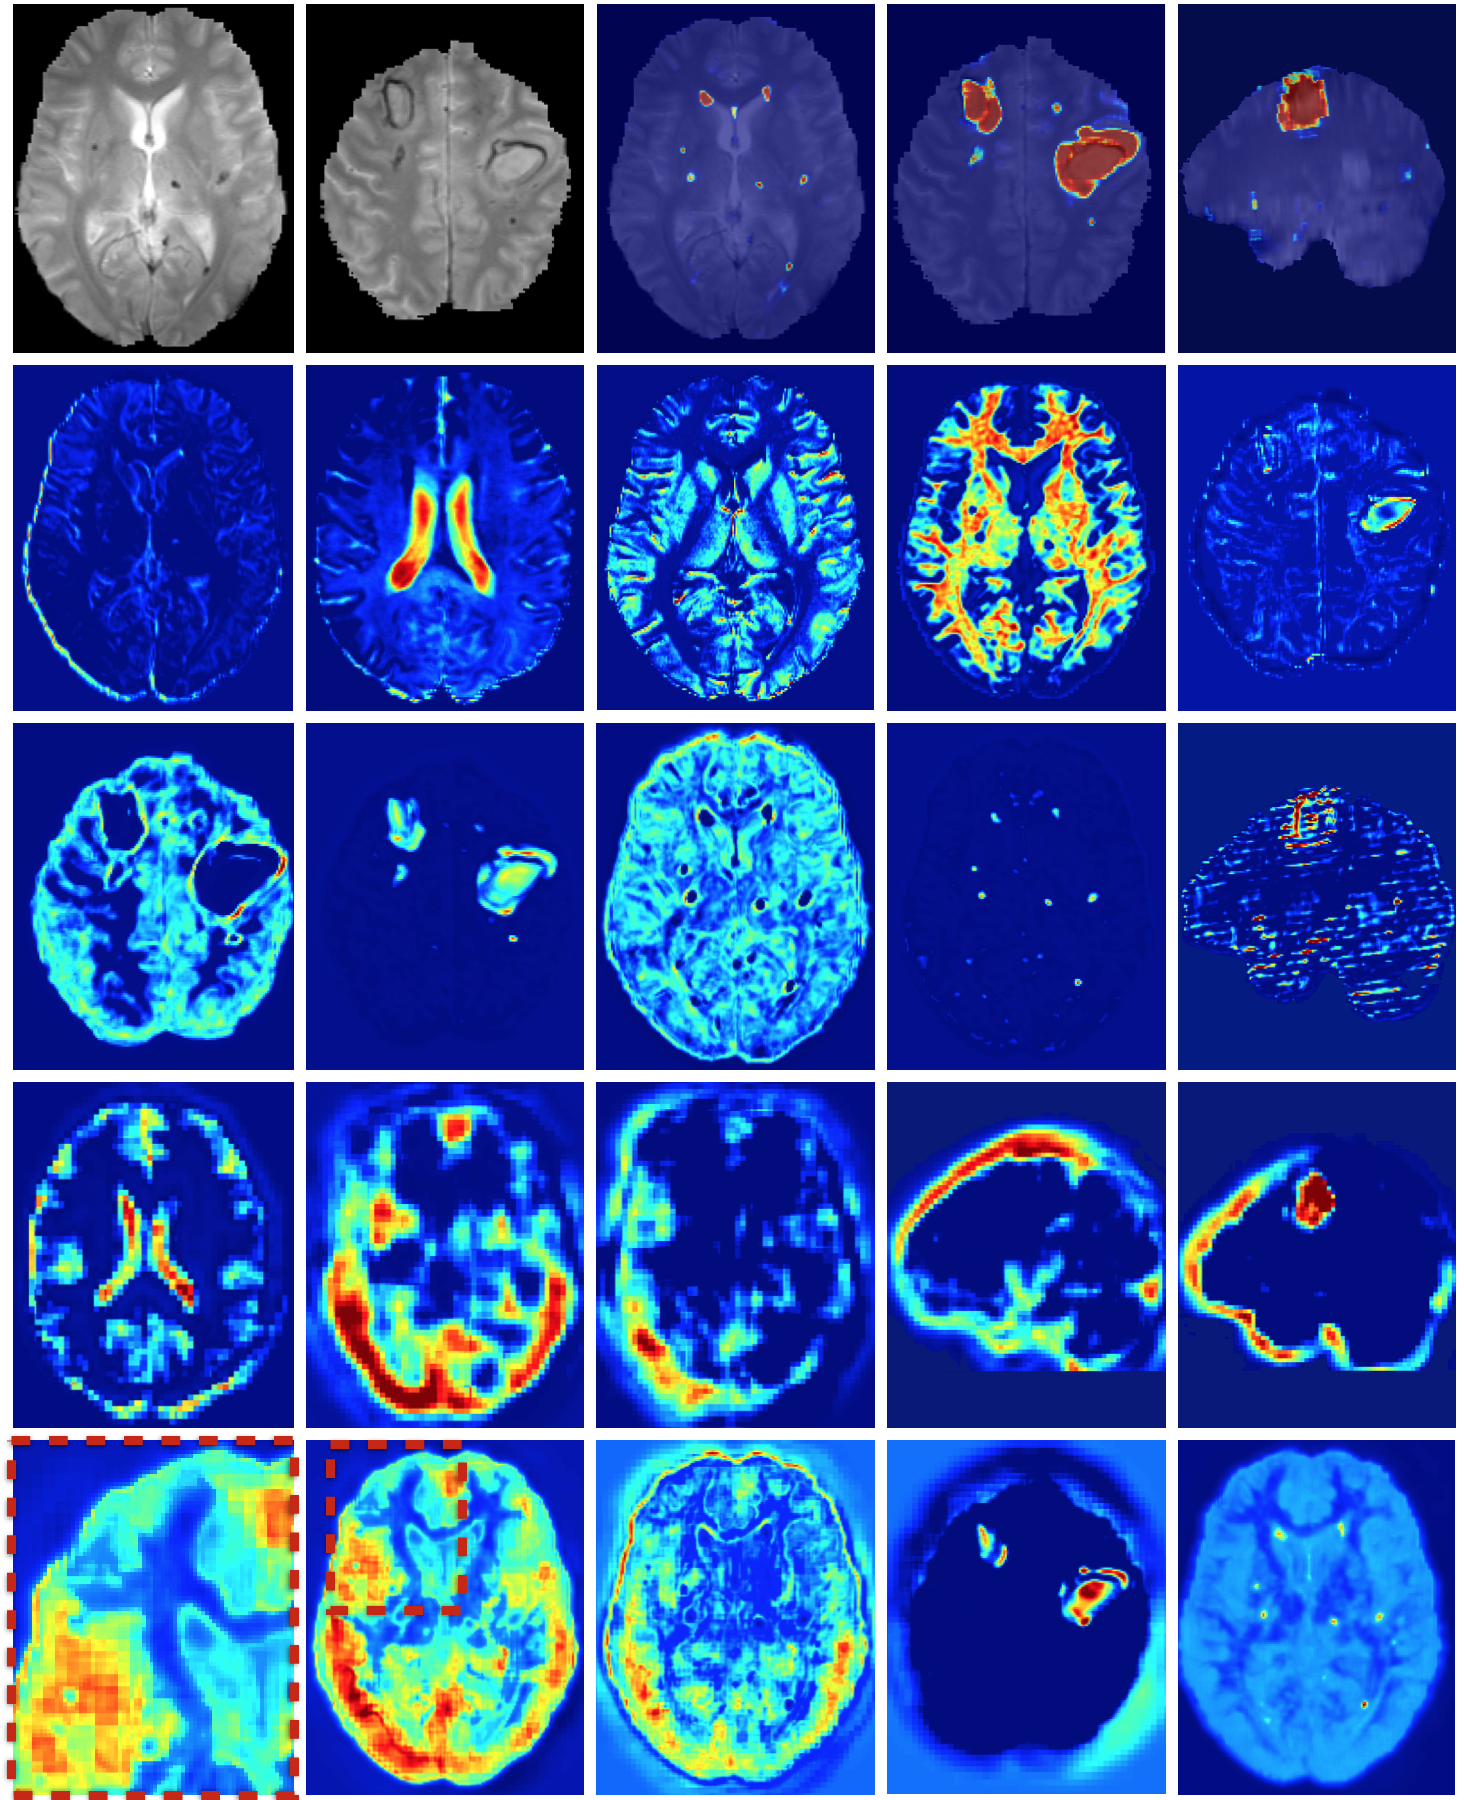
\includegraphics[clip=true, trim=0pt 0pt 0pt 0pt, width=1.0\textwidth]{figures/discussion/featureMapsFigure.png}
\end{subfigure}
\vspace{-5pt} %takes away some white space before the caption
\caption{(First row) GE scan and DeepMedic's segmentation. (Second row) FMs of earlier and (third row) deeper layers of the first convolutional pathway. (Fourth row) Features learnt in the low-resolution pathway. (Last row) FMs of the two last hidden layers, which combine multi-resolution features towards the final segmentation.}
\label{fig:featureMaps}
\end{figure}
%\vspace{-1pt} %takes away some white space after figure